\documentclass{article}

\usepackage{amsmath, amsfonts, amsthm} 
\usepackage{listings}
\usepackage{graphicx}
\usepackage{float}
\usepackage{subfigure}
\usepackage{geometry}

\geometry{
	paper=a4paper, 
	top=2.5cm,
	bottom=2.5cm, 
	left=2.5cm, 
	right=3cm,
	headsep=0.75cm, 
}
\title{ME424 HW6}
\author{Zhuang Yulun 11811126}
\date{\today}

\begin{document}

\maketitle

\section{}
Given
\begin{align*}
    X =
    \begin{bmatrix}
        X_1&X_2&X_3
    \end{bmatrix}^T\\
    \Sigma_X = 
    \begin{bmatrix}
        2&0&\sigma_{13}\\
        0&2&\sigma_{23}\\
        \sigma_{31}&\sigma_{32}&2
    \end{bmatrix}
\end{align*}
\subsection{}
\begin{align*}
    W\sim N(
    \begin{bmatrix}
        0\\0
    \end{bmatrix}
    ,
    \begin{bmatrix}
        2&0\\0&2
    \end{bmatrix}
    )    
\end{align*}
Given Z = 10.

\begin{align*}
    \mu_{W|Z=10} &= \mu_W+\Sigma_{WZ}\Sigma_Z^{-1}(10-\mu_Z)\\
    &=
    \begin{bmatrix}
        0\\0
    \end{bmatrix}
    +
    \begin{bmatrix}
        1\\1
    \end{bmatrix}
    2^{-1}*10\\
    &=
    \begin{bmatrix}
        5\\5
    \end{bmatrix}\\
    \Sigma_{W|Z=10}&=\Sigma_X-\Sigma_{XZ}\Sigma_Z^{-1}\Sigma_{ZX}\\
    &=
    \begin{bmatrix}
        3/2&-1/2\\
        -1/2&3/2
    \end{bmatrix}
\end{align*}
If I observed Z = -10 instead, the conditional mean of W will be negative according to the formula above.
On the other hand, $\Sigma_{WZ}$ shows that W is positive correlated with Z, and $\Sigma^{-1}_Z$ shows that the measurement of Z has little noisy.
Thus, the conditional mean of W is likely to be negative if Z was observed negative.

\subsection{}
$X_1$ is independent of $X_2$ because $X_1$ and $X_2$ are jointly Gaussian and $E(X_1X_2^T)=E(X_1)E(X_2)^T=0$, $Cov(X_1,X_2)=0$.
\\
Define $$Q=(W|Z=10)$$
We have
\begin{align*}
    Q \sim N(
        \begin{bmatrix}
            5\\5
        \end{bmatrix}
        ,
        \begin{bmatrix}
            3/2&-1/2\\
            -1/2&3/2
        \end{bmatrix}
    )
\end{align*}
Since $Cov(Q_1,Q_2)=-1/2$, they are not independent.\\
If $\sigma_{13}=\sigma_{31}=0$ then $Cov(Q_1,Q_2)=0$, so they are independent.

\subsection{}
The probability density function for $W|Z=10$ is
\begin{equation*}
    g(x)=\frac{1}{2\pi |\Sigma|^{-\frac{1}{2}}}\exp^{-\frac{1}{2}(X-\mu)^T\Sigma(X-\mu)}
\end{equation*}
The MATLAB code is shown below.
\begin{lstlisting}
    X = [linspace(0,10,50);linspace(0,10,50)];
    Y = zeros(50,50);
    mu = [5;5];
    sigma = [3/2,-1/2;-1/2,3/2];
    g = @(x,mu,sigma) 1./(2*pi*det(sigma)^(1/2))*exp(-1/2*(x-mu)'*sigma^(-1)*(x-mu));
    for i = 1:size(X,2)
        for j = 1:size(X,2)
            Y(i,j) = g([X(1,i);X(1,j)],mu,sigma);
        end
    end
    surf(X(1,:),X(2,:),Y);
    colormap('jet');
    xlabel('X1');ylabel('X2');
    zlabel('Probability Density');    
\end{lstlisting}
\begin{figure}[H]
    \centering
        \textsf{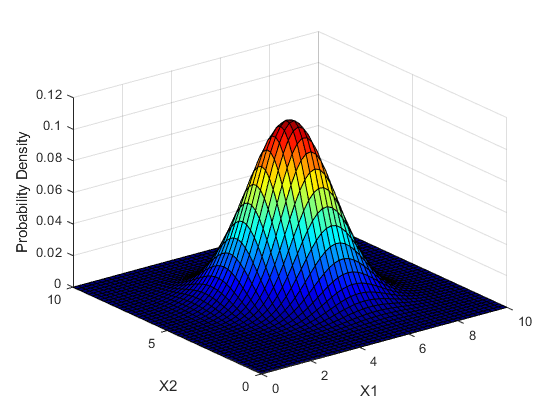
\includegraphics[width=0.6\columnwidth]{hw6-1.png}}
        \caption{PDF for W|Z = 10}
        \label{fig: 1}
\end{figure}

\section{}
\subsection{}
\begin{itemize}
    \item [i]
    $$
    \begin{matrix}
        x_1&1&2\\
        p(x_1|X_2=-1,X_3=3)&\frac{2}{7}&\frac{5}{7}
    \end{matrix}
    $$
    \item [ii]
    \begin{align*}
        &
        \begin{matrix}
            x_1,x_3&1,3&2,2&2,3\\
            p(x_1,x_3|X_2=-1)&\frac{1}{4}&\frac{1}{8}&\frac{5}{8}
        \end{matrix}\\
        &P(X_3=3|X_2=-1)=\frac{7}{8}\\
        &p(x_1|X_2=-1,X_3=3)=\frac{p(x_1,x_3|X_2=-1)}{P(X_3=3|X_2=-1)}\\
        &
        \begin{matrix}
            x_1&1&2\\
            p(x_1|X_2=-1,X_3=3)&\frac{2}{7}&\frac{5}{7}
        \end{matrix}
    \end{align*}
\end{itemize}

\subsection{}
\begin{align*}
    \hat{X_1}_{MMSE} &= E(x_1|X_2 = -1,X_3 = 3)\\
    &=\frac{12}{7}
\end{align*}
\section{}
When $\mu = [1,2]^T$,
\begin{align*}
    \mu^{(1)}_{X|Y=1}&=\mu_x+\Sigma_{XY}\Sigma_Y^{-1}(1-\mu_Y)\\
    &=1+(-1)\times\frac{1}{2}\times(1-2)\\
    &=\frac{3}{2}
\end{align*}
When $\mu = [2,1]^T$,
\begin{align*}
    \mu^{(2)}_{X|Y=1}&=\mu_x+\Sigma_{XY}\Sigma_Y^{-1}(1-\mu_Y)\\
    &=2
\end{align*}
Thus,
\begin{align*}
    X_{MMSE}&=\mu^{(1)}_{X|Y=1}Prob(\mu=\mu^{(1)})+\mu^{(2)}_{X|Y=1}Prob(\mu=\mu^{(2)})\\
    &=1.9
\end{align*}
\section{}
Given
\begin{align*}
    X&\sim N(
        \begin{bmatrix}
            1\\2
        \end{bmatrix}
        ,
        \begin{bmatrix}
            1&-1\\-1&2
        \end{bmatrix}
    )\\
    V&\sim N(0,3)\\
    Z&=HX+V,\ where\ H=[1\ 2]
\end{align*}
\subsection{}
We have
\begin{align*}
    E(Z)&=HE(X)+E(V)\\
    &=5\\
    Cov(Z)&=Cov(HX+V,HX+V)\\
    &=HCov(X)H^T+Cov(V)\\
    &=8\\
    Coc(X,Z)&=Cov(X,HX+V)\\
    &=Cov(X)H^T\\
    &=\begin{bmatrix}
        -1\\3
    \end{bmatrix}\\
    Cov(Z,X)&=Cov(HX+V,X)\\
    &=HCov(X)\\
    &=[-1\ 3]
\end{align*}
Thus
\begin{align*}
    E(X|Z=4)&=\mu_X+\Sigma_{XZ}\Sigma_Z^{-1}(4-\mu_Z)\\
    &=\begin{bmatrix}
        9/8\\13/8
    \end{bmatrix}\\
    Cov(X|Z=4)&=\Sigma_X-\Sigma_{XZ}\Sigma_Z^{-1}\Sigma_{ZX}\\
    &=\begin{bmatrix}
        7/8&-5/8\\
        -5/8&7/8
    \end{bmatrix}
\end{align*}

\subsection{}
I need update the mean and covariance of X given Z = 4.
\begin{align*}
    \begin{Bmatrix}
        E(X)\\Cov(X)
    \end{Bmatrix}
    \underrightarrow{measurement\ update}
    \begin{Bmatrix}
        E(X|Z=4)\\Cov(X|Z=4)
    \end{Bmatrix}
\end{align*}
According to Kalman formula, 
\begin{align*}
    K&=\Sigma_XH^T(H\Sigma_XH^T+\Sigma_V)^{-1}\\
    &=
    \begin{bmatrix}
        -1/8\\3/8
    \end{bmatrix}
    \\
    E(X|Z=4)&=\mu_X+K(4-H\mu_X)\\
    &=
    \begin{bmatrix}
        9/8\\13/8
    \end{bmatrix}\\
    Cov(X|Z=4)&=(I-KH)\Sigma_X\\
    &=
    \begin{bmatrix}
        7/8&-5/8\\
        -5/8&7/8
    \end{bmatrix}
\end{align*}


\end{document}